\documentclass[12pt, a4paper]{article}

\usepackage[utf8]{inputenc}
\usepackage[T1]{fontenc}
\usepackage[margin=2.5cm]{geometry}
\usepackage{graphicx}
\usepackage{listings}
\usepackage{xcolor}
\usepackage{hyperref}
\usepackage{parskip}

\definecolor{codebg}{RGB}{244,243,236}
\definecolor{keywordcolor}{RGB}{0,147,108}
\definecolor{stringcolor}{RGB}{180,80,0}

\lstdefinestyle{json}{
    backgroundcolor=\color{codebg},
    basicstyle=\ttfamily\small,
    keywordstyle=\color{keywordcolor},
    stringstyle=\color{stringcolor},
    breaklines=true,
    frame=single,
    framesep=6pt,
    rulecolor=\color{gray!30},
    showstringspaces=false,
    tabsize=2,
}

\title{\textbf{Event Planner} \\ \large Project Report}
\author{}
\date{\today}

\begin{document}

\maketitle
\tableofcontents
\newpage

% -----------------------------------------------------------------------
\section{Overview}

This is a full-stack event planning application built with Node.js / Express
on the backend and React / TypeScript on the frontend.
It allows users to create and manage events, register attendees, and issue
tickets that link attendees to events.
The backend exposes a REST API backed by MongoDB Atlas via Mongoose, deployed
as a serverless function on Vercel.
The frontend is a single-page application using React Router v7 for
client-side routing, a global store via React Context, and no UI framework
--- all styles are handwritten CSS using custom properties.
Data flows through typed service functions that call \texttt{apiFetch}, a
thin wrapper around the browser \texttt{fetch} API.

% -----------------------------------------------------------------------
\section{Data Model}

The application uses three MongoDB collections: \texttt{events},
\texttt{attendees}, and \texttt{tickets}. A ticket acts as a join document,
holding a reference to both an event and an attendee, along with a type
(\texttt{standard} or \texttt{vip}) and a status (\texttt{active} or
\texttt{cancelled}). A unique compound index on \texttt{(event, attendee)}
prevents duplicate registrations.

\begin{figure}[h]
    \centering
    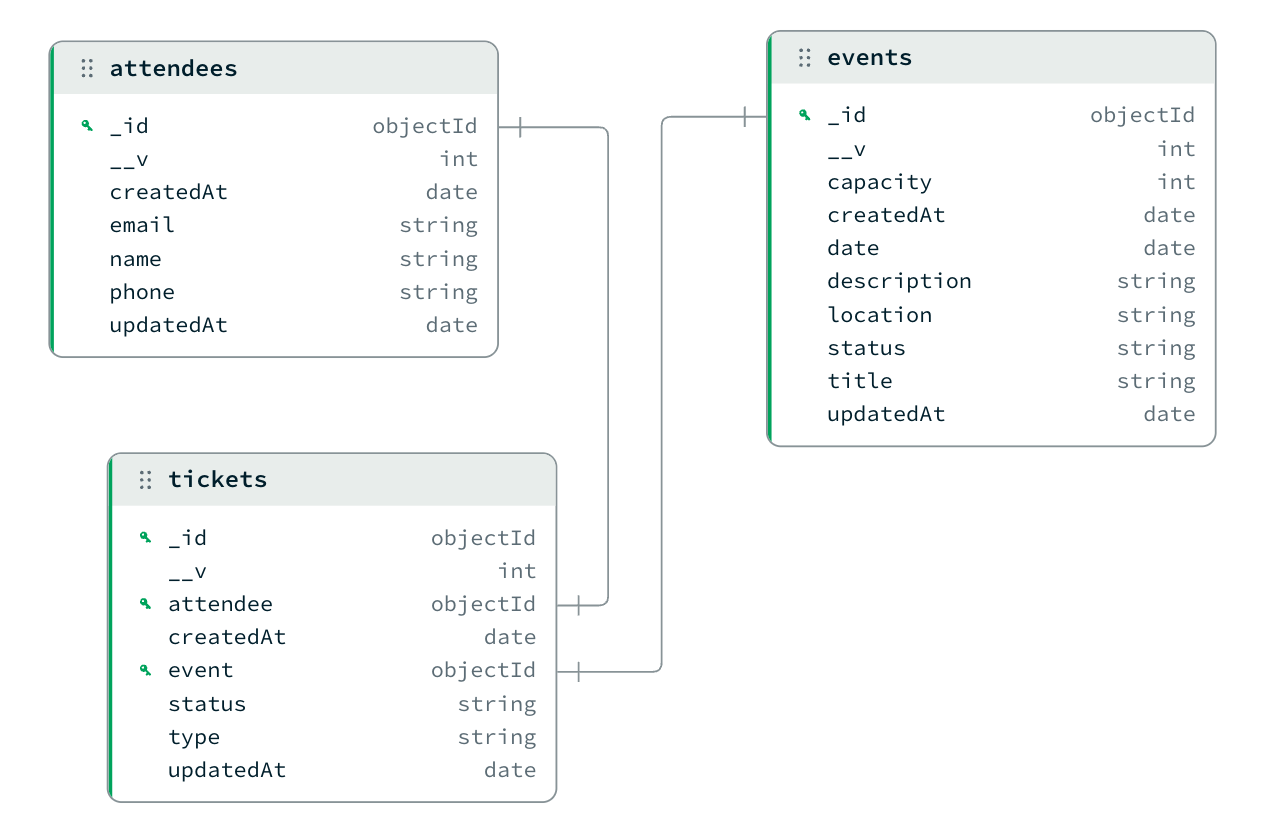
\includegraphics[width=0.85\textwidth]{erd.png}
    \caption{Entity Relationship Diagram}
\end{figure}

% -----------------------------------------------------------------------
\section{API Endpoints}

\subsection{POST /api/events}

Creates a new event. \texttt{title}, \texttt{date}, and \texttt{status} are
required. \texttt{status} must be one of \texttt{upcoming}, \texttt{ongoing},
\texttt{completed}, or \texttt{cancelled}. When an event is updated to
\texttt{cancelled}, all its active tickets are automatically cancelled via a
bulk update.

\textbf{Request body:}
\begin{lstlisting}[style=json]
{
  "title": "Tech Conference 2025",
  "description": "Annual developer meetup",
  "date": "2025-09-15T09:00:00.000Z",
  "location": "Malmo",
  "capacity": 200,
  "status": "upcoming"
}
\end{lstlisting}

\textbf{Response 201:}
\begin{lstlisting}[style=json]
{
  "success": true,
  "data": {
    "_id": "664a1f...",
    "title": "Tech Conference 2025",
    "description": "Annual developer meetup",
    "date": "2025-09-15T09:00:00.000Z",
    "location": "Malmo",
    "capacity": 200,
    "status": "upcoming",
    "createdAt": "2025-04-25T10:00:00.000Z",
    "updatedAt": "2025-04-25T10:00:00.000Z"
  }
}
\end{lstlisting}

\subsection{POST /api/tickets}

Registers an attendee to an event by creating a ticket. Both \texttt{event}
and \texttt{attendee} must be valid ObjectIds referencing existing documents
--- the endpoint verifies both before inserting. \texttt{type} must be
\texttt{standard} or \texttt{vip}.

\textbf{Request body:}
\begin{lstlisting}[style=json]
{
  "event": "664a1f...",
  "attendee": "664b2e...",
  "type": "standard"
}
\end{lstlisting}

\textbf{Response 201:}
\begin{lstlisting}[style=json]
{
  "success": true,
  "data": {
    "_id": "664c3d...",
    "event": "664a1f...",
    "attendee": "664b2e...",
    "type": "standard",
    "status": "active",
    "createdAt": "2025-04-25T10:05:00.000Z",
    "updatedAt": "2025-04-25T10:05:00.000Z"
  }
}
\end{lstlisting}

% -----------------------------------------------------------------------
\section{Challenges}

Designing an effective central store was one of the more complex parts of the
frontend. Getting the Context API to avoid unnecessary re-renders across
collections required careful use of \texttt{useMemo} per collection, so that
updating events, for example, would not re-render components that only consume
attendees.

A time-consuming deployment issue turned out to be a forgotten step: the
MongoDB Atlas cluster had IP access restricted to a specific address, and the
Vercel deployment IP was not whitelisted. The API kept timing out with no
clear error until the network access list in the Atlas dashboard was updated
to allow connections from all IPs.

\end{document}
